\nsection{OSN 4 Способы объектно-реляционного отображения для классов и атрибутов, бинарных и N-арных ассоциаций, классов ассоциаций, иерархий наследования. Примеры применения этих способов. Моделирование схемы реляционной базы данных с помощью диаграммы классов.}

\textbf{Реляционная} схема данных и объектная модель оперируют разными понятиями, из-за чего необходима специальная работа по объектно-реляционному отображению. Отображение возможно в обе стороны: в \textbf{прямую} (от классов к таблицам) и в обратную (от таблиц к классам). Отображение может быть таким, что для конкретной модели классов строится соответствующая только этой модели схема реляционной базы данных. Такой подход назовём зависимым от модели. Альтернативный подход – \textit{универсальный} – отличается тем, что схема реляционной базы данных подходит для любой исходной модели классов.

В качестве универсального рассматривается мэппинг Амблера, хорош универсальностью: схема не изменится (в отличие от ORM далее), если в исходную модель классов, преобразовываемую в реляционную схему, добавить/удалить класс или связь. Недостаток мэппинга Амблера в том, что операции с экземплярами, со связями, со значениями громоздки (применим только для малых моделей). Так при создании объекта нужно определить набор атрибутов его класса, создать слоты для хранения значений атрибутов в объекте. 
Переводить модель классов в схему БД предлагается в 3 этапа: отобразить классы в таблицы, отобразить ассоциации и отобразить связи обобщения. 

\textbf{ORM-стратегии классов:}

\textbf{1.} Каждый класс переводится в отдельную таблицу, столбцы которой служат для хранения значений
скалярных атрибутов, и каждая запись которой соответствует экземпляру класса. 

\textbf{2.} Уникальный идентификатор устойчивого класса (совокупность атрибутов класса, помеченных ограничением {id}) превращается в первичный ключ таблицы. Если явного идент-ра нет, то он добавляется.

\textbf{ORM-стратегии атрибутов:} 

\textbf{1.} Атрибут мощностью 1 или 0..1 (со значением скалярного типа) может быть переведён в один столбец таблицы класса. В зависимости от практических соображений один атрибут может быть переведён в несколько столбцов. Например, вместо того, чтобы хранить адрес клиента в одном столбце, можно разбить адрес на части (город, улица, дом, № квартиры и т. п.) и хранить каждую часть в отдельном столбце. \textbf{2.} Для атрибутов мощностью * заводится отдельная таблица, каждая запись которой хранит значение атрибута и ссылку (во внешнем ключе) на запись об экземпляре класса, к которому относится значение. 

\textbf{3.} Для атрибутов с точной верхней границей мощности можно не заводить отдельную таблицу, а добавить несколько столбцов (адрес1, адрес2, адрес3, …). 

\textbf{4.} Для выводимых атрибутов можно не заводить столбцов. Их значения можно не хранить, а вычислять. 

\textbf{5.} Значения статических атрибутов следует хранить в отдельной служебной таблице. Таблица для статических атрибутов может иметь несколько строк и 4 столбца: \textbf{<}id, имяКласса, имяАтрибута, значение\textbf{>}. На основе этого решения можно получить таблицу для статических атрибутов с мощностью *.

При отображении ассоциаций можно пытаться экономить и не создавать дополнительные таблицы для хранения соединений между устойчивыми объектами за счет объединения нескольких таблиц в одну или за счёт добавления внешних ключей в таблицы. \textbf{Стратегии ORM бинарных ассоциаций:} 

\textbf{1.}«1 к 1му» – возможны различные решения, лучше создать общую таблицу для 2х классов. Столбцы – совокупность атрибутов. Пример: класс <<Персона>>1<--->1<<Свид-во о рождении>>; 

\textbf{2.} «1 к 0..1» – внешний ключ добавляется к таблице необязательного класса. Вообще говоря, можно было бы использовать тот же прием, что и в «1 к 1», но получающаяся таблица будет «разреженной» – в некоторых записях будут пустые поля. Пример: класс <<Персона>>1<--->0..1<<Паспорт>> (не у всех есть паспорт) В <<Паспорт>> добавляется внешний ключ idПерсоны. 

\textbf{3.} «0..1 к 0..1» – работают оба выше указанных решения, с поправкой на изменившуюся мощность, но также рекомендуется ещё одно – отдельная таблица для связи. Пример: <<Автомобиль>>0..1<--->0..1<<Прицеп>> 

\textbf{4.} «* к *» – для ассоциации заводится отдельная таблица. Ее столбцы – внешние ключи для таблиц классов, связанных ассоциацией. Основной ключ – набор из обоих столбцов.

\textbf{ORM N-арной ассоциации:} Требуется служебная таблица для хранения связи. Например, в случае тернарной (N=3) ассоциации служебная таблица состоять из внешних ключей для каждой из трёх таблиц, полученных при ORM классов, а все её столбцы в наборе дадут её первичный ключ.

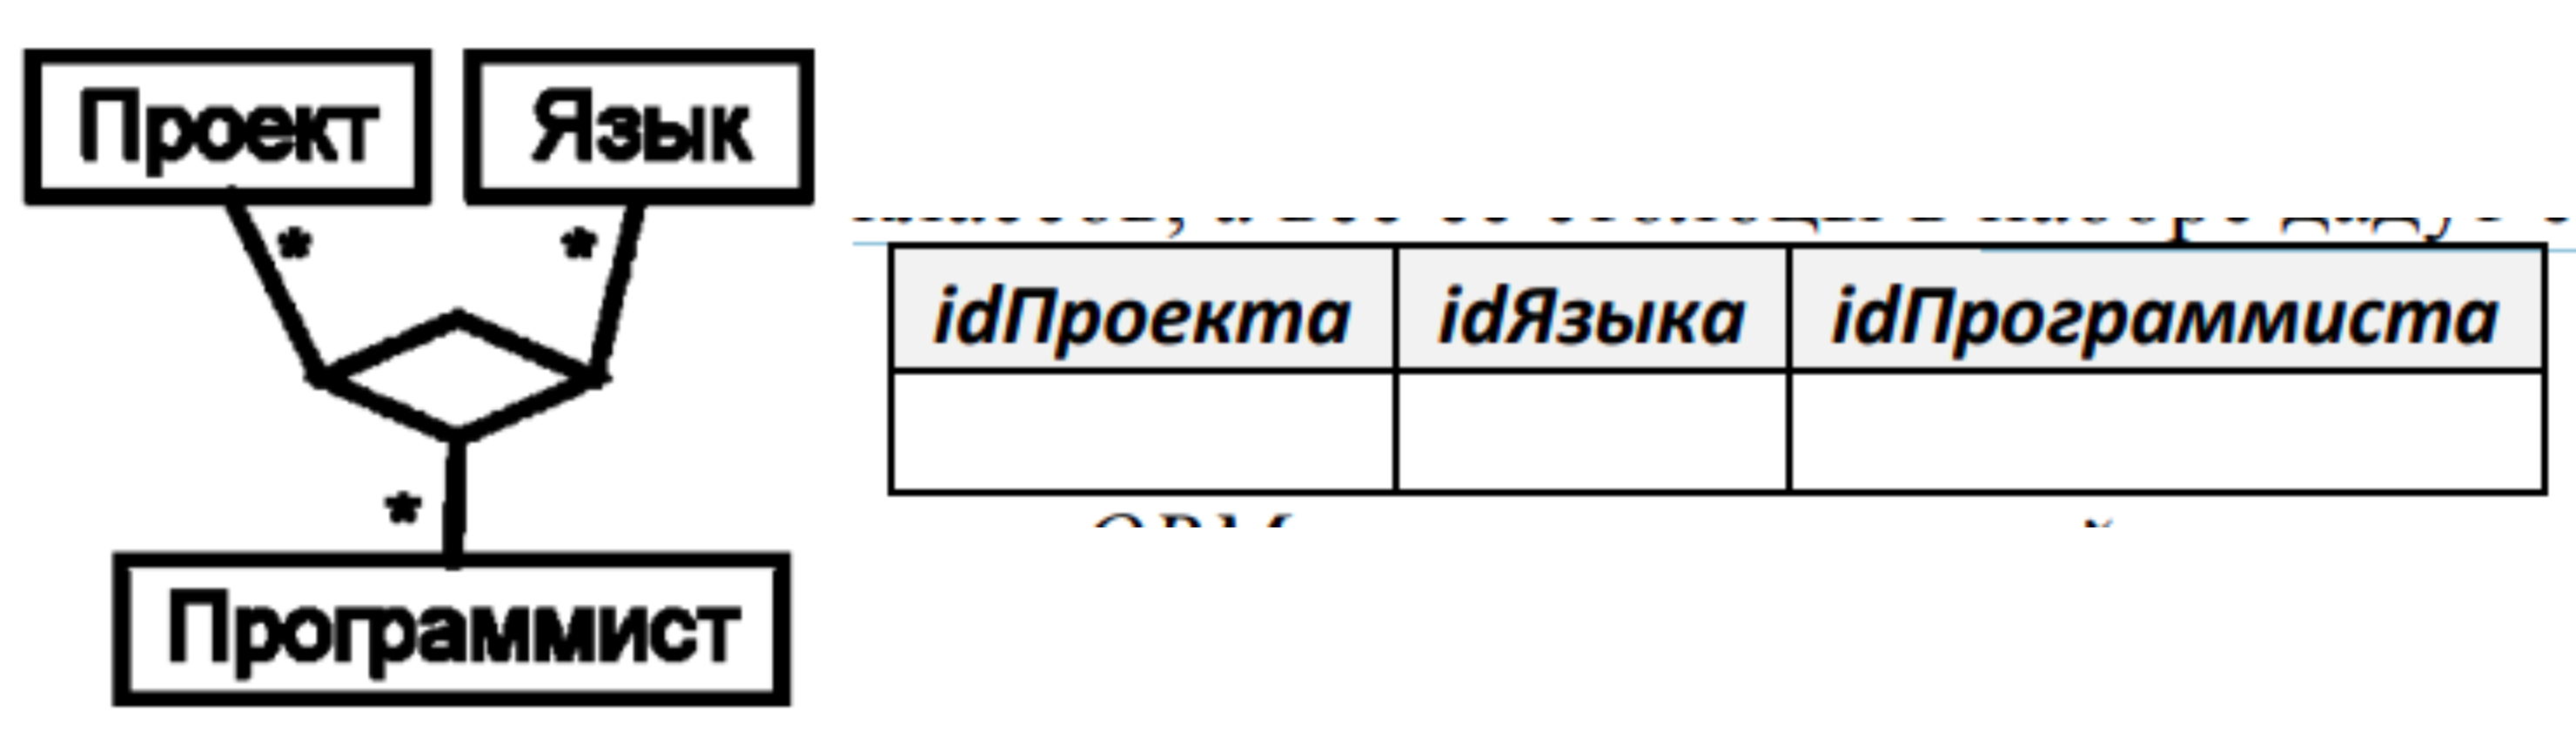
\includegraphics[scale=0.05]{pics/4_1.png}

\textbf{ORM классов-ассоциаций:} Атрибуты класса-ассоциации добавляются либо в создаваемую для связи таблицу, либо (если дополнительная таблица не требуется) в ту таблицу, куда добавляется внешний ключ, либо в общую таблицу (при слиянии).

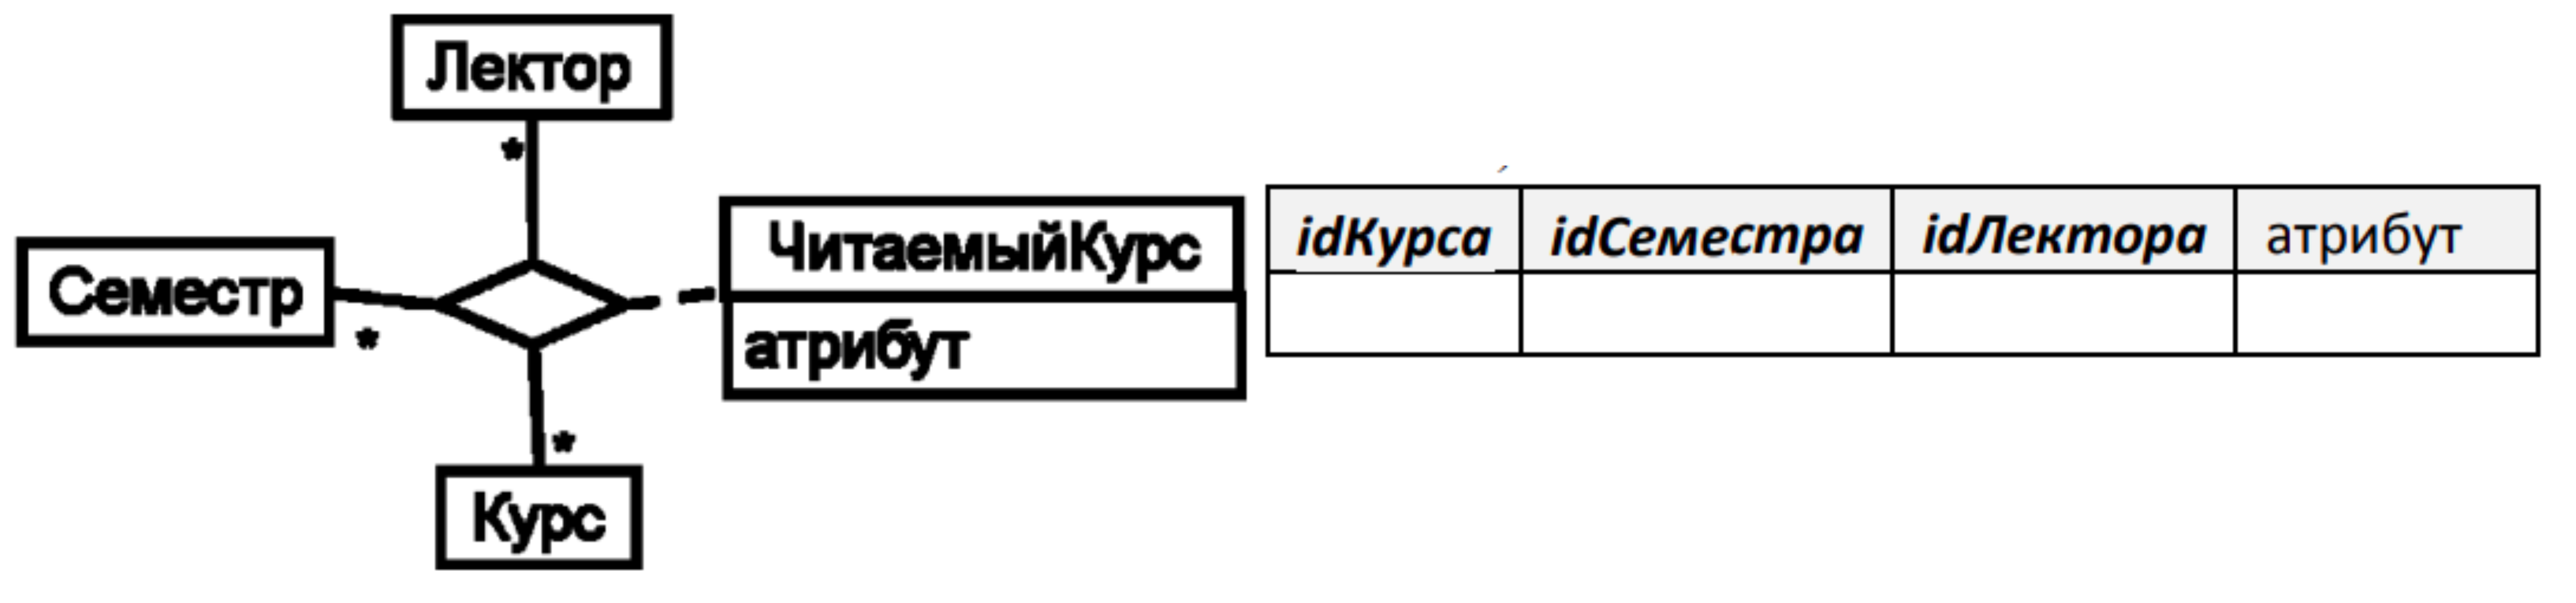
\includegraphics[scale=0.05]{pics/4_2.png}

Подводя итог ORM ассоциаций, перечислим использованные выше стратегии: слияние таблиц, добавление внешнего ключа, отдельная таблица для связи.

\textbf{ORM обобщения (наследования):}
Какой именно способ выбрать диктуют соображения эффективности (скорость в обмен на объем памяти). Рассмотрим на примере. Заметим, что класс Person – абстрактный, а класс StudentEmployee имеет двух предков.
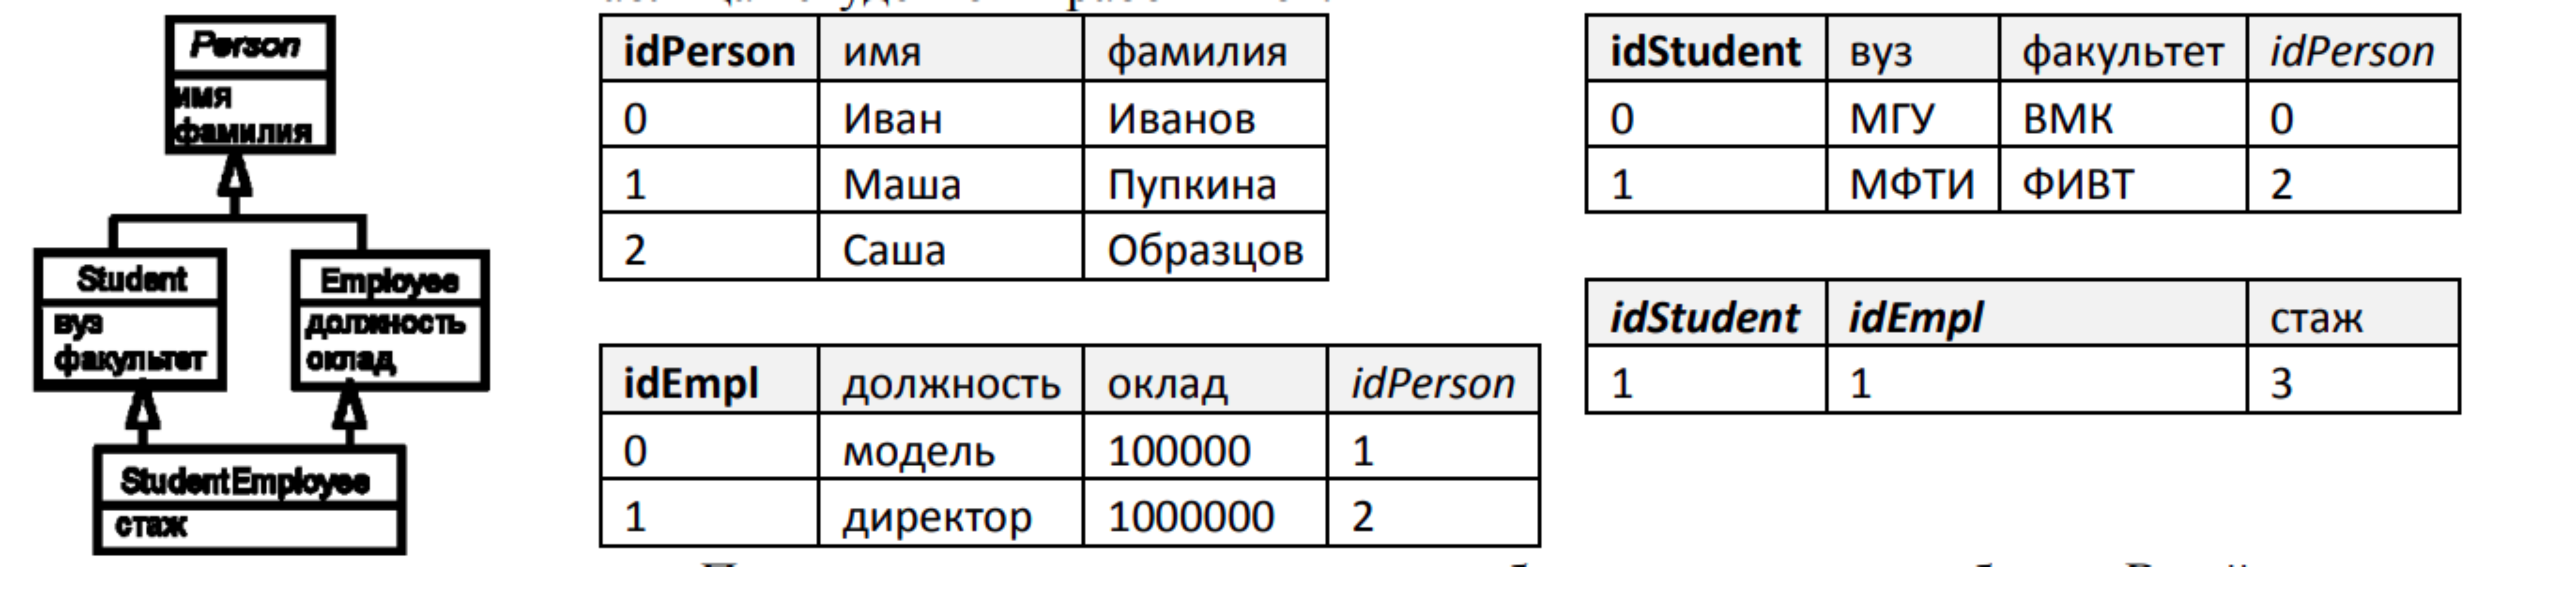
\includegraphics[scale=0.05]{pics/4_3.png}

\textbf{Стратегии}:

1) для каждого класса своя таблица (на картинке справа);

2) для всей иерархии наследования одна таблица (все поля в одной таблицы, добавятся в ней булевские isStudent и isEmployee, но будут пустые поля, например, не все обладают стажем);

3) таблицы только для конкретных (не абстрактных) классов (Person мы убираем, а поля имя и фамилия храним в Student и Employee);

4) таблицы только для различных конкретных классов (две таблицы: Student и Employee, в каждой стаж, в первой флаг isEmployee, во второй-isStudent).

Перейдём к тому, как с помощью диаграмм классов можно моделировать схемы БД. «pk, fk» (столбец, входящий в первичный и во внешний ключ помечается двумя стереотипами) – другой способ записи «pk» «fk». Связи между таблицами моделируются как ассоциации между классами. Связь является идентифицирующей, если первичный ключ связанной таблицы включает в себя её внешний ключ. В остальных случаях она не идентифицирующая. Для отображения ограничений целостности связь может моделироваться композицией. С её помощью описывается тот факт, что связанные записи одной таблицы следует удалить при удалении записи из другой таблицы (рядом с которой стоит «ромбик» композиции). Рассмотрим примеры из модели системы обработки заказов. Диаграмма с устойчивыми классами приведена ниже (и как мы её преобразовали в схему БД, нижняя схема)
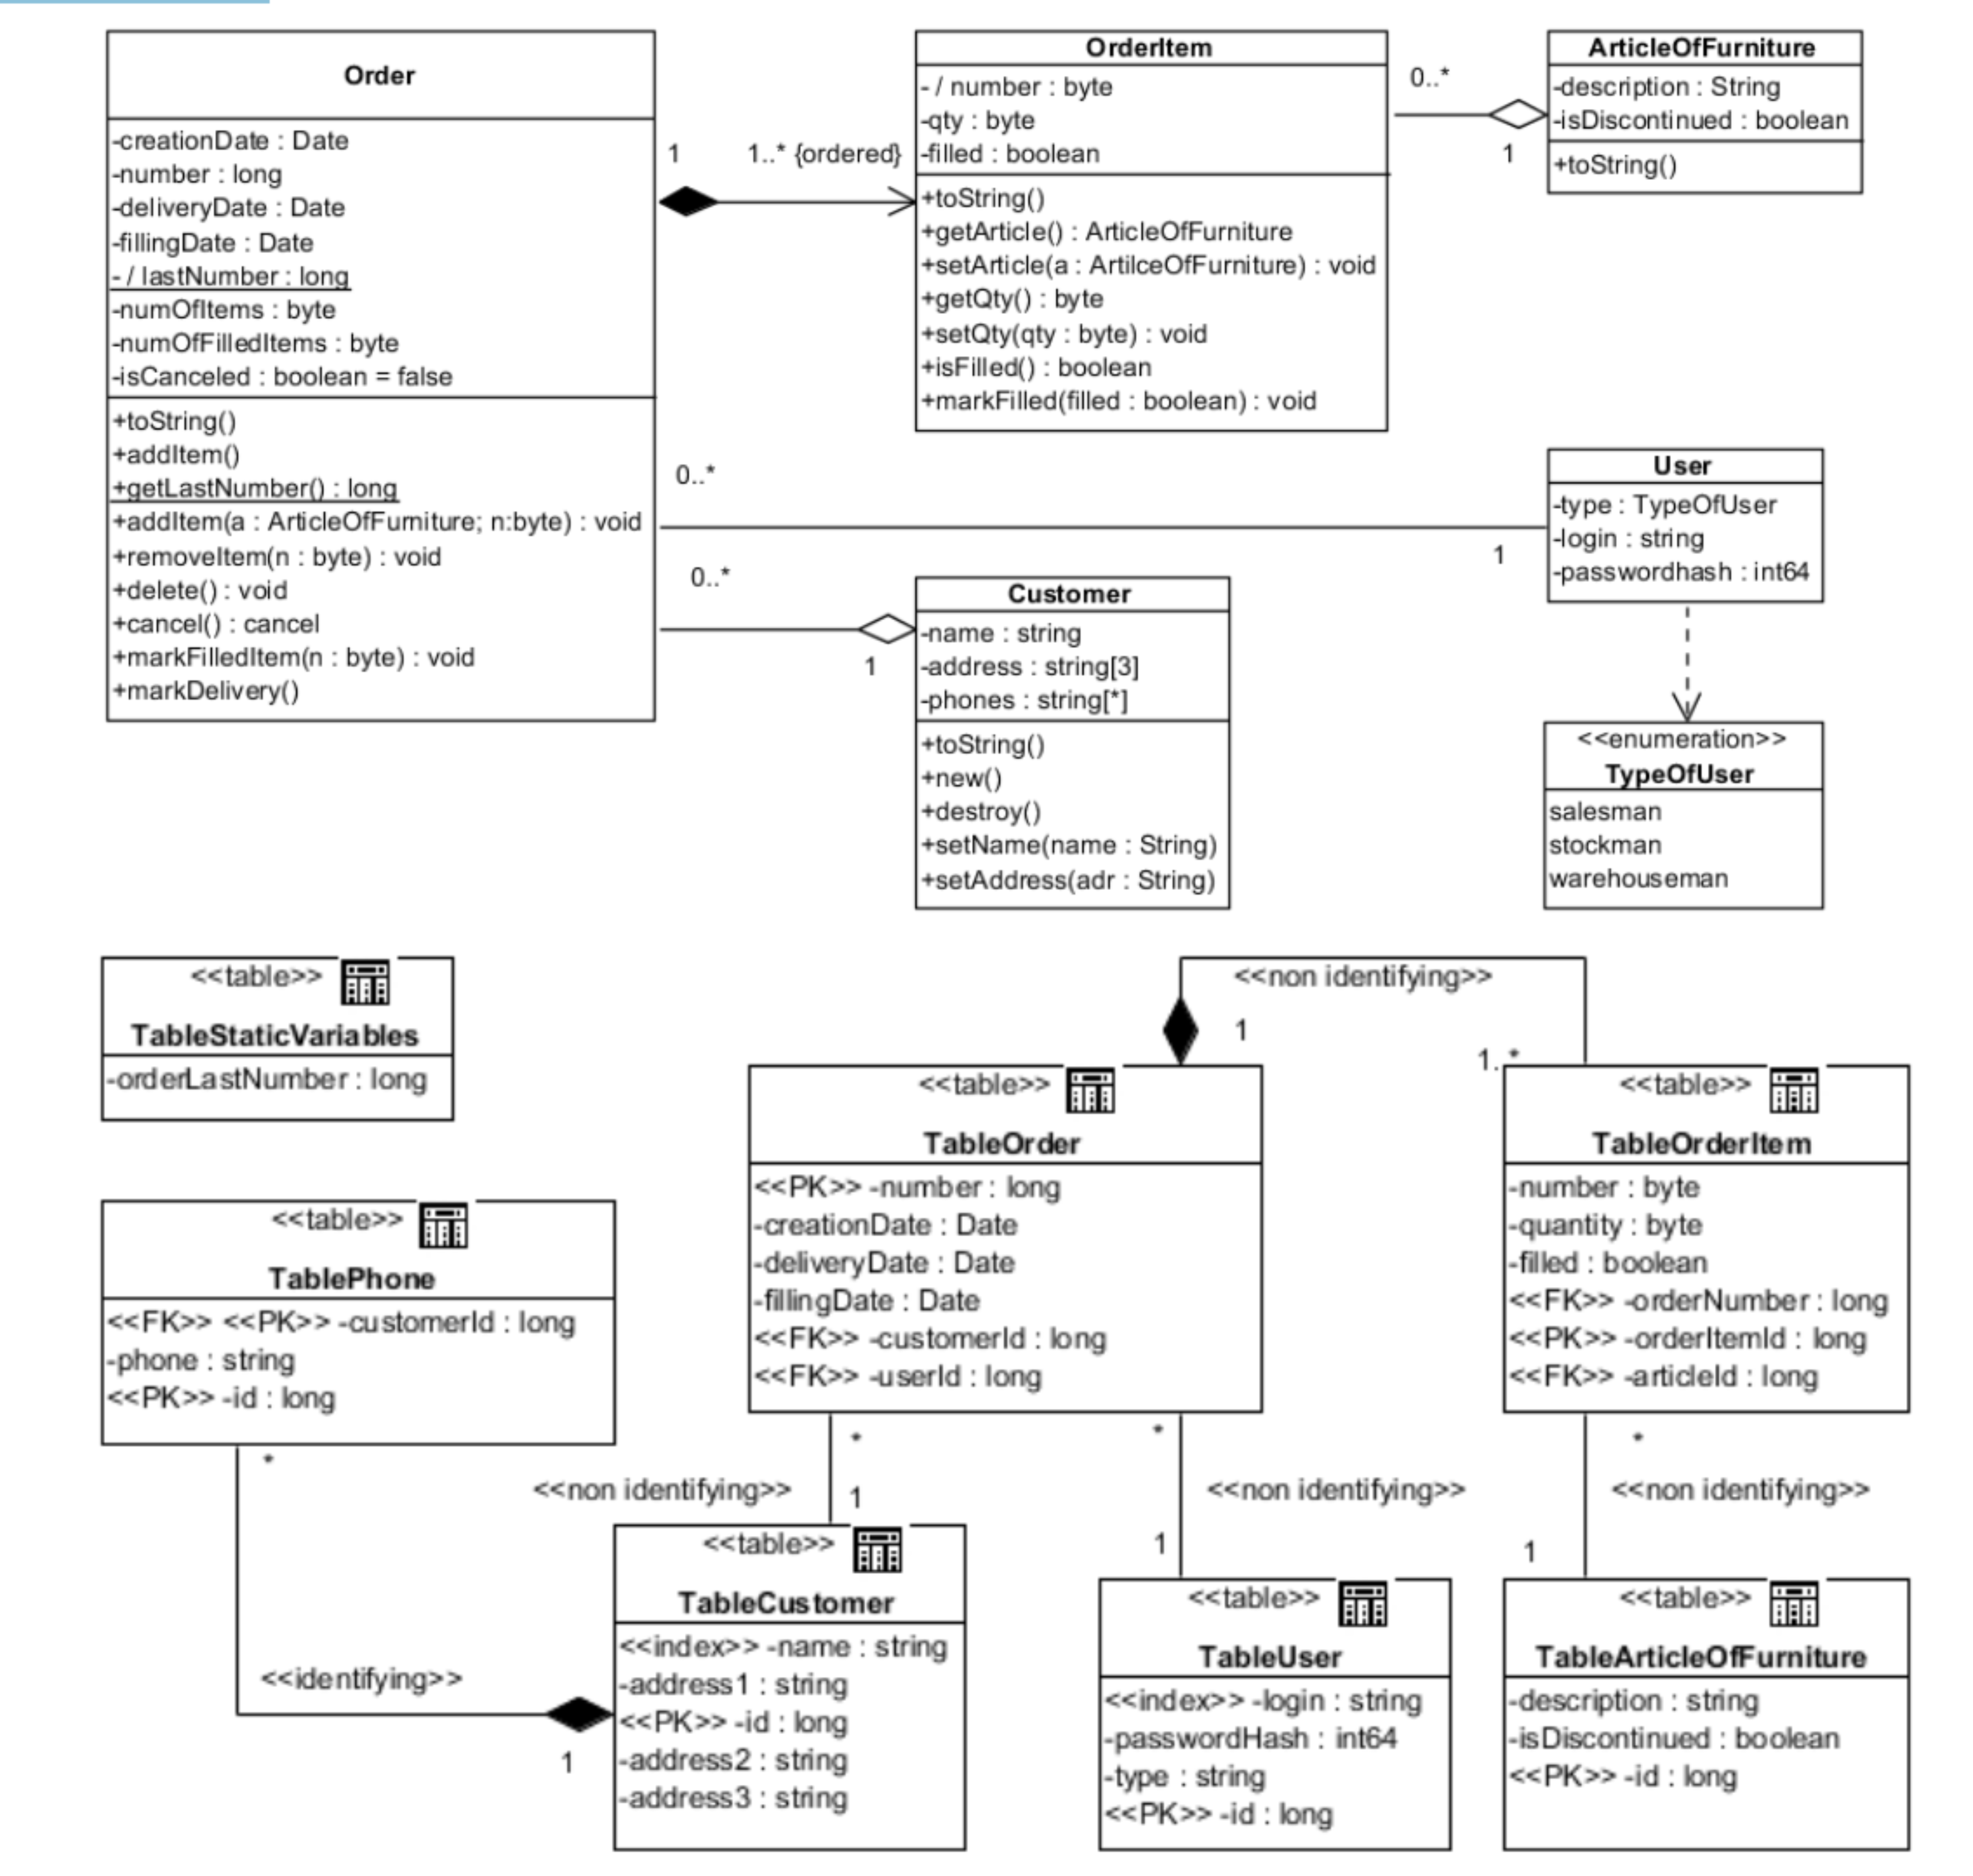
\includegraphics[scale=0.06]{pics/4_4.png}

